\documentclass{llncs}

\usepackage[english]{babel}
%\usepackage[tight]{subfigure}
%\usepackage{floatrow}
\usepackage{graphicx}
%\usepackage{amsmath}
%\usepackage{multirow}
%\renewcommand*\arraystretch{1.25} % extra vertical space in cells
\usepackage{amsmath}

\begin{document}

\title{A Framework for Modelling Thin Objects: \\ from Meshing to Shell Finite Element Method}
%\author{Olivier Comas, St\'ephane Cotin and Christian Duriez}
%\institute{INRIA, Alcove team, Lille, France}

\maketitle

\begin{abstract}

\end{abstract}

\section{Introduction}

Human body is composed of various deformable anatomical structures. 
Realistic modeling of organ deformations is a challenging research field that leads the way to numerous clinical applications including: medical training and rehearsal systems, patient-specific planning of surgical procedure and per-operative guidance based on simulation.
In all these cases, the clinician needs fast update of the deformation model to obtain a real-time display of the computed deformations.  
To realize this kind of interactive systems, one face the trade-off problem between accuracy of the model and the need of fast computations. 

An other key challenge of real-time human soft-tissue modeling is the variousness of the mechanical behaviors. 
It seems unrealistic to target a unique model for all tissues even if there are obvious advantages to make maximum use of optimized generic models.
Yet most of previous work focus on volume models that are able to capture the behavior of volume organs like liver \cite{} or brain tissues \cite{}.
In contrast, this paper seeks to propose a solution for simulating, in real-time, deformation of thin anatomical structures, whose volume is negligible compared to their surface area.
Examples of such anatomical structures include hollow structures, like the wall of blood vessels or the colon but also the envelope of volume organs, like the capsule of Glisson.


In the following of this paper, we present a framework for realistic and real-time simulation of thin organs.
Our method, presented in section \ref{sec:model} is based on shell theory and computes the internal forces using Finite Element Modeling (FEM) on curved triangles.
The design of the elements relies on a polynomial interpolation that is also use to capture the interactions with other models, including volume models.
We also present an automatic process to obtain meshes from image based reconstruction in an attempt to optimize  the computation using fewer elements  (see section \ref{sec:mesh}).
The benefits of our approach (meshing of a curved surface, fast computation and possible interactions with volume models) are illustrated using various examples presented in section \ref{sec:results}. 


\section{A physical model for thin structures}
\label{sec:model}
\subsection{Related work}

Development of a satisfactory physical model that runs in real-time but produces visually convincing animation of thin objects is challenging. Rather than resorting to shell theory which involves the most complex formulations in continuum mechanics, previous works have often relied on discrete formulations. Early approaches only considered in-plane deformation, and often relied on mass-spring models. More recent works have considered adding bending through angular springs. For instance Wang et al.~\cite{Wang07} successfully used a network of linear and angular springs to describe bending and twisting of catheters and guidewires in an interventional radiology simulator. Yet, such models are limited in their ability to describe certain behaviour, as they do not rely on continuum mechanics. Another limitation of such models is the difficulty to derive spring stiffness (in particular for angular springs) from elastic properties (Young's modulus and Poisson's ratio). For these reasons, other approaches have been proposed. 

Continuum mechanics provides many formulations able to accurately describe stresses occurring within thin objects. Most of them fall into one of the following two categories: plate theory or shell theory. Those theories have been a subject of interest in the mechanical community for decades. The difference between these two kinds of structures is very well explained by Liu et al.~\cite{Liu03} and can be summarized by the fact that plate bending elements can only carry transversal loads while shells can undergo more complex deformations. Considering the wide range of shapes and solicitations that can be applied to hollow organs, a thin plate model would not correctly capture their deformation and therefore a shell formulation was retained.

\subsection{Co-rotational triangular shell model}

A complete description of our co-rotational triangular shell finite element model is available in one of our previous publication \cite{Comas2010ISBMS}. Therefore we will only remind briefly the key points. We improved and extended a plate model first introduced by Przemieniecki \cite{Przemieniecki68} to a co-rotational formulation. Co-rotational approaches offer a good trade-off between computational efficiency and accuracy by allowing small deformations but large displacements. Once combined with an in-plane membrane formulation we obtain an accurate, yet computationally efficient, shell finite element method featuring both membrane and bending energies. 

\subsubsection{Triangular elastic membrane}

The element stiffness matrix $\textbf{K}_e$ can be computed as follows:

\begin{equation}
\textbf{K}_e = \int_v \textbf{J} \boldsymbol{\chi} \textbf{J}^{T} dV
\end{equation}
where $\textbf{J}$ is the strain-displacement matrix and $\boldsymbol\chi$ embodies the material's behaviour. The stiffness matrix in the global frame is eventually obtained using the rotation matrix of the element: $\textbf{K} = \textbf{R}^{T} \textbf{K}_e \textbf{R} $ where $\textbf{R}$ describes the rotation of the (triangular) element with respect to its initial configuration.

\subsubsection{Triangular plate bending}

\begin{figure}
\centering
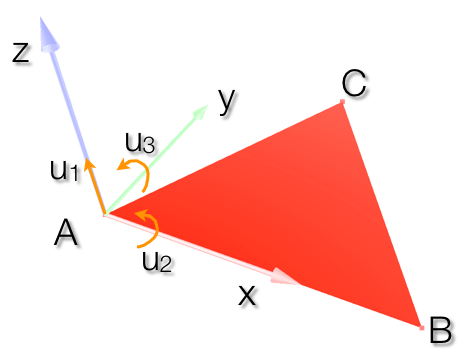
\includegraphics[height=5cm]{images/bending}
\caption {The different degrees of freedom $u$ of a triangular thin plate in bending are illustrated above.}
\label{fig-triangle}
\end{figure}

To calculate the stiffness matrix for the transverse deflections and rotations shown on figure \ref{fig-triangle}, we start with the assumed deflection $u_z$ of the form
\begin{equation}
 u_z = c_1 + c_2x + c_3y + c_4x^2 + c_5xy + c_6y^2 + c_7x^3 + c_8xy^2 + c_9y^3
\label{eq-deflection}
\end{equation} 

where $c_1$, \ldots , $c_9$ are constants. Let us define the vector $\textbf{u} = \left\{u_1 u_2 \ldots u_9 \right\} $ of the displacements and slopes at the three corners of the triangular plate using the following notations:
\begin{equation}
u_1 = (u_z)_{x_1,y_1} \hspace{1cm} u_2 = \left(\frac{\partial u_z}{\partial y}\right)_{x_1,y_1} \hspace{1cm} u_3 = - \left(\frac{\partial u_z}{\partial x}\right)_{x_1,y_1}
\end{equation} 
and so on for the two other vertices.
We then can derive a matrix $C$ such as $\textbf{u} = \textbf{Cc}$ where $\textbf{c} = \left\{c_1 c_2 \ldots c_9 \right\} $.

We can calculate the strains from the flat-plate theory using:
\begin{equation}
e_{xx} = -z \frac{\partial^2u_z}{\partial x^2}
\end{equation} 
\begin{equation}
e_{yy} = -z \frac{\partial^2u_z}{\partial y^2}
\end{equation} 
\begin{equation}
e_{xy} = -2z \frac{\partial^2u_z}{\partial x \partial y}
\end{equation} 

Symbolically this may be expressed as $\textbf{e} = \textbf{Dc}$ where $\textbf{D}$ derives from equation~\ref{eq-deflection} and the above relations. Noting that $\textbf{c} = \textbf{C}^{-1}\textbf{u}$, we have:
\begin{equation}
\textbf{e} = \textbf{DC}^{-1}\textbf{u} = \textbf{bu}
\end{equation} 
where the strain-displacement matrix $\textbf{b} = \textbf{DC}^{-1}$. 
The stiffness matrix $\textbf{K}_e$ for an element is then classically obtained from
\begin{equation}
\textbf{K}_e = \int_v \textbf{b}^{T} \boldsymbol\chi \textbf{b} dV
\end{equation} 
where $\boldsymbol\chi$ is the material matrix. The stiffness matrix in the global frame is eventually obtained using the rotation matrix of the element as in the membrane case. 

\section{Meshing a curved surface}
\label{sec:mesh}
\subsection{Related work}

A key component of finite element methods is the mesh of the simulated object being used. While a sufficient number of elements is needed to accurately describe the geometry, too many of them will yield a computationally expensive simulation and solving the system in real-time may no longer be possible. Literature about volumic mesh generation algorithms is fairly dense. However, there are only a few that are concerned about the generation of meshes over curved surfaces. One of the most widely used techniques for the creation of surface meshes is the plane to surface transformation method \cite{Zienkiewicz71}, mesh is first generated on a two-dimensional domain and then mapped onto the surface. If this method gives reasonably good meshes on smooth surfaces, the results are usually quite poor with more complex curved surfaces. The finite elements may be generated directly on the curved surfaces based on the advancing front technique \cite{Lo85,Lau96}. The main issue with this approach is that an analytical description of the geometry is needed, which is not the case in medical simulation. Another method consists of using an a priori error estimator to build an adaptive mesh generation \cite{Baumann97}. However, the tolerance of this indicator should be chosen depending on the desired accuracy of the finite element solution, and therefore requires some knowledge about the problem in order to choose an effective tolerance. In \cite{Bechet02} the authors start from an existing triangular mesh created with a CAD software and refine and smooth the mesh based on element quality and surface curvature. While all those methods allow their authors to get satisfactory meshes over curved surfaces according to their needs, they all make use of flat elements to mesh geometries and do not generate actual shells. 

\subsection{A mechanically-driven method to mesh curved surfaces with shells}

Indeed, one main difference between shell and plate elements is that the rest shape of the former can describe a curved surface. We propose to take this crucial feature into account to optimise the meshing process. While many flat triangles are often required to describe highly curved surfaces, fewer triangular shell elements are needed to describe the given geometry with the same precision since they can be naturally curved. In the following we assume that we have a high resolution triangular mesh obtained from a binary segmented image of the organ we want to simulate (via a Marching Cube algorithm for instance). Our goal is to create a mesh featuring the optimal number of shell elements while staying as close as possible to our targeted geometry. 

Therefore we need to insure that the distance between the surface of our shell-based mesh and the targeted high resolution mesh will be minimal. To our knowledge the only tool available to measure error between two surfaces is the Hausdorff distance \cite{Klein96,Cignoni98}. As a reminder the Hausdorff distance between two meshes is the maximum between the two so-called one-sided Hausdorff distances:

\begin{equation}
d_{\mathrm{H}}(X,Y) = \max \left\{ \sup_{x \in X} \inf_{y \in Y} d(x,y), \sup_{y \in Y} \inf_{x \in X} d(x,y) \right\} \enspace .
\end{equation}
where $d()$ is the Euclidian distance between two points. Since the curved surface of each shell must be taken into account in the computation of the Hausdorff distance, a finer mesh is created by adding vertices on the surface of each element. We first sample the flat surface of each element by recursively dividing each triangle into four smaller ones and the deflection of each new vertex is computed using (\ref{eq-deflection}). We then use this new mesh that samples the actual surface described by the shells to compute the Hausdorff distance with the targeted high resolution mesh. The same process of subdivision allows us to render each shell as a curved triangle (Fig.~\ref{fig-shell} ). 

\begin{figure}
\centering
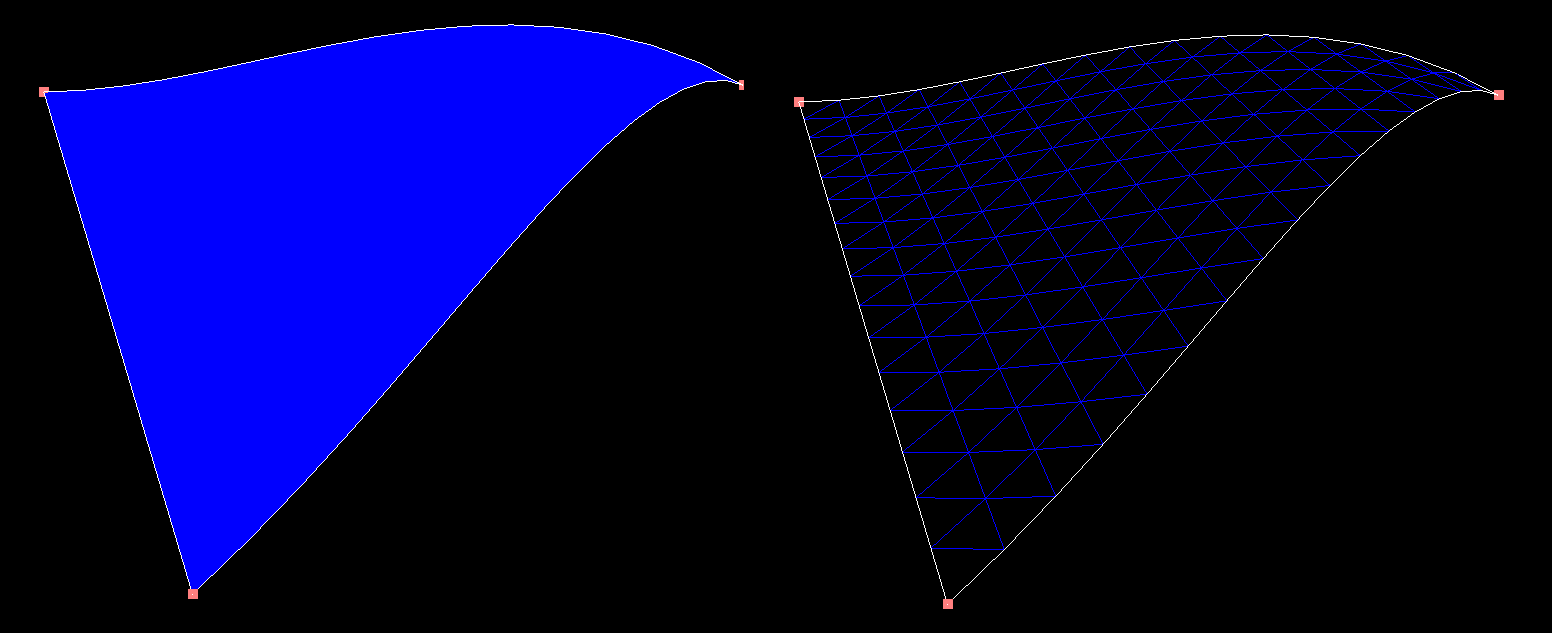
\includegraphics[height=4cm]{images/shell_curvature}
\caption {The triangle formed by the three vertices of the shell has been recursively subdivided 3 times and the deflection of each new vertex was computed according to the same deflection function used in our shell finite element formulation. Sampling the actual surface of the shell allows rendering and more accurate Hausdorff distance computation. }
\label{fig-shell}
\end{figure}

The first step in the process of generating a shell-based mesh is an aggressive decimation of the targeted high resolution mesh. We then apply a heuristic method derived from the work of Saupin et. al \cite{Saupin07} with tetrahedral meshes based on very simple geometrical rules. For each node of the coarse mesh, we find the three closest triangles on the high resolution mesh and we move the node to the barycenter of the three centres of mass of those triangles. This technique locally smooths the surface of the mesh while converging towards the desired high resolution mesh. At each iteration of this algorithm we measure the error with the target using the Hausdorff distance and the process is stopped when the required precision has been reached. A simple example is shown Fig. \ref{fig-cylinder} and \ref{fig-cylinderResults} to illustrate the method. 

\begin{figure}
\centering
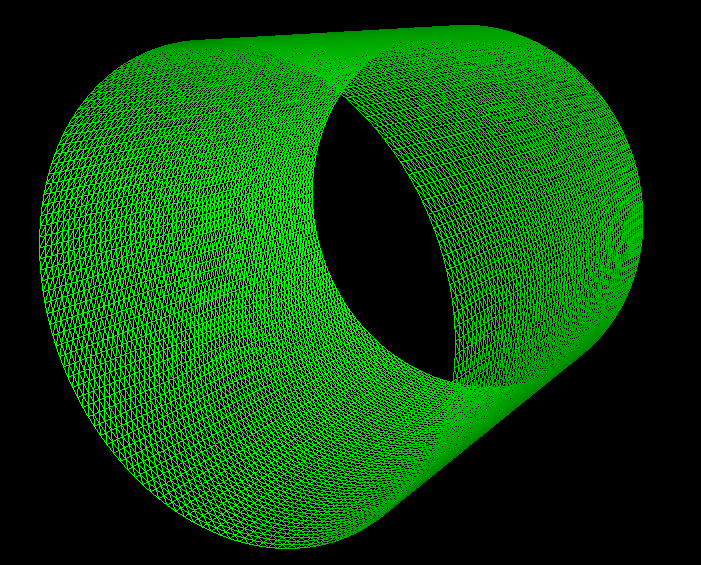
\includegraphics[height=4cm]{images/cylinderHighWireframe}
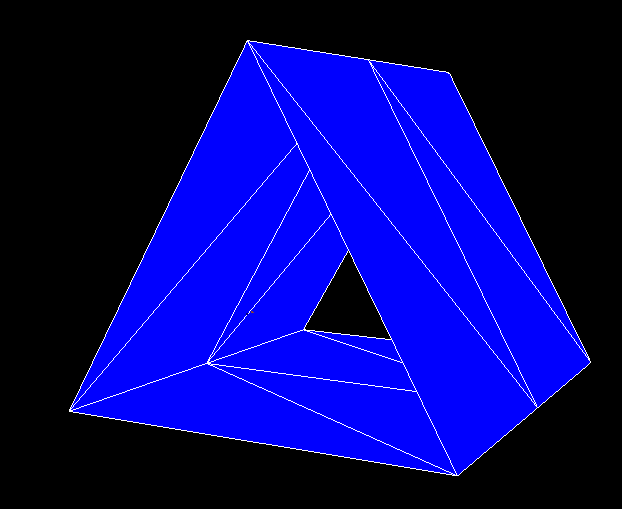
\includegraphics[height=4cm]{images/cylinderLow}
\caption {Illustration of our method on a simple example. The target is the high resolution cylinder mesh (left) and the start point is a very coarse mesh approximating the shape of a cylinder (right).}
\label{fig-cylinder}
\end{figure}

\begin{figure}
\centering
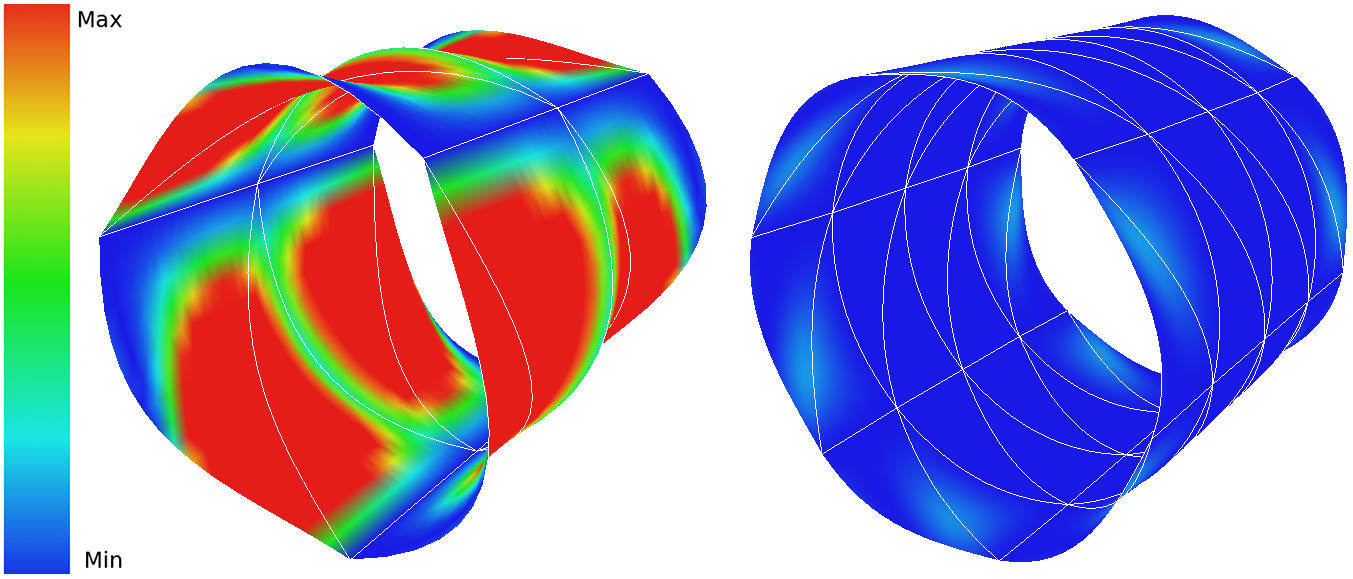
\includegraphics[height=4cm]{images/cylinderResults2}
\caption {(Left) Hausdorff distance colour map of the coarse mesh rendered with shells. (Right) Hausdorff distance colour map after one iteration of our algorithm. We can notice that differences with the target mesh have been subtantially reduced.}
\label{fig-cylinderResults}
\end{figure}

\section{Results}
\label{sec:results}
\subsection{Meshing of anatomical structures (error maps)}



\subsection{Deformations}
\subsubsection{Computation times on 3 examples}
\subsubsection{Coupling between tetrahedra and shells for more advanced modelling}
\begin{figure}
\centering
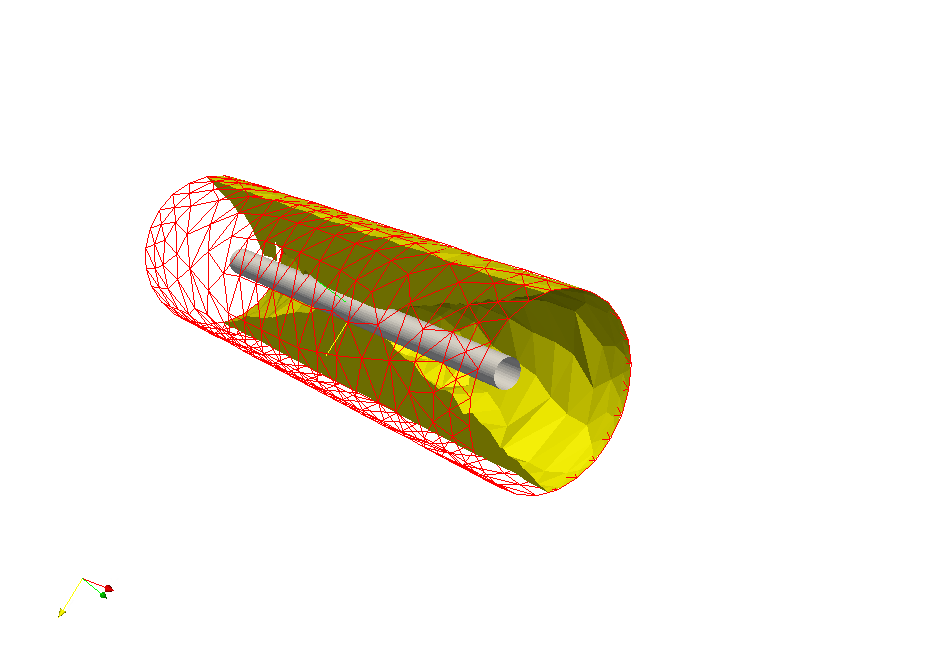
\includegraphics[height=4cm]{images/stent_begin.png}
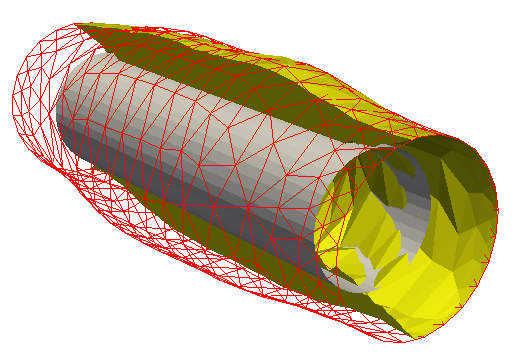
\includegraphics[height=4cm]{images/stent_end.png}
\caption {Avant... Apres...}
\label{fig-stent}
\end{figure}


\section{Conclusion}
\section*{Acknowledgments}

\bibliographystyle{splncs}
\bibliography{bibliography}

\end{document}